\documentclass[8pt]{beamer}
% \usepackage{graphicx}
% \usepackage[all,cmtip]{xy}
\usepackage{tikz}
\usepackage{tikz-cd}
\usepackage{qtree}
% \usepackage{diagxy}
\usepackage{amsfonts}
\usepackage{amssymb}
\usepackage{amsmath}
\usepackage{amscd}
\usepackage{amsthm}
\usepackage{mathpartir}
\usepackage{bbm}
%\usepackage{pictexwd,dcpic}
\usepackage[mathcal]{euscript}
\usepackage[utf8]{inputenc}
%\usepackage[T1]{fontenc}
\usepackage{lmodern}
%\usepackage{setspace}
%\usepackage{mathpartir}
% \usepackage{proof}
%\setstretch{1}
\title{Structural Foundations for Abstract Mathematics}
\author{Dimitrios Tsementzis and Hans Halvorson}
\date{May 5, 2013}
\usetheme{Copenhagen}
\begin{document}
\def\2{\mathcal}
\def\7{\mathbb}
\begin{frame}


%% Focus: the appropriate criterion of identity --- evil, stupid

\maketitle


\end{frame}
\begin{frame}

\newenvironment{proenv}{\only{\setbeamercolor{local structure}{fg=green}}}{}
\newenvironment{conenv}{\only{\setbeamercolor{local structure}{fg=red}}}{}  
\newenvironment{neuenv}{\only{\setbeamercolor{local structure}{fg=yellow}}}{}


What no foundation can give us:
\begin{itemize}
\item<con@1-> Certainty
\end{itemize}

\bigskip
What foundations need not give us:
\begin{itemize}
\item<neu@1-> Ontological reduction
\end{itemize}

\bigskip
What set theory gives us:
\begin{itemize}
\item<pro@1-> Common language in which \emph{all} mathematics can be encoded:
  $\forall ,\exists ,\in,\dots$
\item<pro@1-> Dispute resolution (is CH true?)
\item<pro@1-> Guidance in gray areas (can we assign a measure to all
  subsets of $\mathbb{R}$?)
\item<pro@1-> Clarity about inferential relations and commitments
\end{itemize}
\end{frame}

\begin{frame}

\def\7{\mathbb}
\newenvironment{conenv}{\only{\setbeamercolor{local structure}{fg=red}}}{}  

When set theory throws sand in our eyes:
\begin{itemize}
\item<con@1-> The Doplicher-Roberts theorem
\item<con@1-> Two theories cannot be equivalent unless their models
  are isomorphic
\item<con@1-> Equivalence is \emph{the} correct notion of ``sameness''
  for categories.
\item<con@1-> Benacerraf: number theory is insensitive to
  set-theoretic details
\item<con@1-> $\7Z\cong 2\7Z$, but there is a set-theoretic predicate
  $P$ such that $P(\mathbb{Z})$ and $\neg P(2\mathbb{Z})$.
$$ P(x)\:  =_{\mathrm{df}} \: 1\in x $$
\item<con@1-> Makkai:
  \begin{quote} ``Let $G$ and $H$ be arbitrary groups, and consider
    the intersection of their underlying sets.''  \end{quote}
\item<con@1-> MacLane:
  \begin{quote} ``\dots as Weyl once remarked, [set theory] contains
    far too much sand.'' \end{quote}
\end{itemize}

\end{frame}


\begin{frame}
  Proposed solutions to the \textbf{sand problem}:

\bigskip

\Tree [.Structuralism Ontological [.Practical [.Informal {Burgess \& Pettigrew} Awodey ] [.Formal ETCS CCFM SFAM ]] ]


\end{frame}

\begin{frame}

  \textbf{Structuralist Thesis:} Mathematics is concerned with the
    relations that objects bear to each other, rather than with what
    these objects \emph{are}.

\bigskip
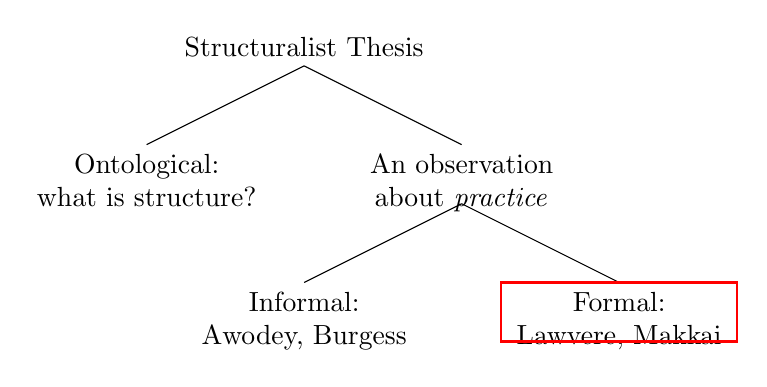
\begin{tikzpicture}
\draw (2,-1) -- (4,0);
\draw (6,-1) -- (4,0);
\draw (6,-1.75) -- (4,-2.75);
\draw (6,-1.75) -- (8,-2.75);
\node[align=center, above] at (4.0,0)%
{Structuralist Thesis};
\node[align=center, below] at (2,-1)%
{Ontological: \\ what is structure?};
\node[align=center, below] at (6,-1)%
{An observation \\ about \emph{practice}};
\node[align=center, below] at (4,-2.75)%
{Informal: \\ Awodey, Burgess };
\node[align=center, below] at (8,-2.75)%
{Formal: \\ Lawvere, Makkai};
\draw [red, thick] (6.5,-2.75) rectangle (9.5,-3.5);
\end{tikzpicture}

\end{frame}


\def\2{\mathcal}

\begin{frame}{Elementary Theory of the Category of Sets}

\begin{tabular}{ccc} \begin{tikzcd}
E_1\times _{E_0} E_1 \arrow{d} \\
E_1 \arrow[transform canvas={xshift=1ex}]{d} \arrow[transform
canvas={xshift=-1ex}]{d}  \\
E_0 \arrow{u} \end{tikzcd}
& \begin{tikzcd}[ampersand replacement=\&]
\& c \arrow{d} \arrow{dl} \arrow{dr} \\
F(i) \& F(j) \& F(k) \end{tikzcd}
\begin{tikzcd}[ampersand replacement=\&]
1\arrow{r}{z} \arrow{dr}{q} \& n \arrow{r}{s} \arrow{d}{u} \& n \arrow{d}{u} \\
\& c \arrow{r}{f} \& c \end{tikzcd}
\end{tabular}

\bigskip
\begin{itemize}
\item Two-sorted theory
\item No Sand: Quantifiers range over objects and arrows, not over elements
\item But: $a\in S\quad \equiv \quad 1\stackrel{a}{\to}S$
\end{itemize}


\end{frame}


\begin{frame}{Category of Categories as the Foundation for
    Mathematics}

Language: $\{ \Delta _0,\Delta _1,\cdot \} \cup \{ \partial _0 ,\partial _1\}$

\bigskip 

\begin{tabular}{ccc}
  $\mathbf{1}$ & $\mathbf{2}$ &  $\mathbf{3}$ \\ \\
$\forall y\exists !z(y\stackrel{z}{\to} x)$ & $\Delta _i(\partial
_j)=\mathbf{2}$ & \\ \\
\begin{tikzcd} \bullet \end{tikzcd}
& \begin{tikzcd}[ampersand replacement=\&] \bullet \arrow{r} \&
  \bullet \end{tikzcd} 
& \begin{tikzcd}[ampersand replacement=\&] \bullet \arrow{r} \arrow{dr}
  \& \bullet \arrow{d} \\
\& \bullet \end{tikzcd}
\end{tabular}

\bigskip
``arrow in $C$'' $\quad \equiv\quad$ ``functor from $\mathbf{2}$ to $A$''








\end{frame}

\begin{frame}{Global foundations}

\begin{tabular}{lllll}
  & Syntax  & Language & Deductive System & Semantics \\
  \hline \hline 
  Set Theory & FOL$_=$ & $\{ \in \}$ & classical + ZFC & cumulative
  hierarchy \\
  ETCS & FOL$_=$ & $\{ \circ ,d_0,d_1,i\}$  & classical + Lawvere &
  CCFM? \end{tabular}

\bigskip

In all cases, $=$ is globally defined

\end{frame}

\frame{ \frametitle{All global foundations say ``stupid'' things}
  \textbf{Claim} Any global foundation will say stupid things.
\begin{itemize}
\item Levels: A set is a structure of level $0$. A mathematical
  structure is of level $n$ (incl. $\infty$) if its natural setting is
  in an $n$-category.
\begin{itemize}
\item e.g.\ Groups are level-$1$ structures, categories are level-$2$
\item e.g.\ Simplicial sets are both level $1$ and level $\infty$
  depending on the context
\end{itemize}
\item Suppose we have two local criteria of identity $\sim_1$ and
  $\sim_2$. We say that $\sim_1$ is \textbf{coarser}
  (resp. \textbf{finer}) than $\sim_2$ if $P \sim_2 Q$ implies $P
  \sim_1 Q$ (resp. $P \sim_1 Q$ implies $P \sim_2 Q$)
  \begin{itemize}
\item This assumes that structures are commensurable, possible up to
  some canonical mapping. e.g. $\mathbb{Q} \hookrightarrow
  \mathbb{R}$.
\end{itemize}
\item ``Lemma'': If $m \geq n$ then the criterion of identity
  $\sim_{\mathcal{S}}$ for a collection (or type) $\mathcal{S}$ of
  structures of level $m$ will be coarser than the criterion of
  identity $\sim_{\mathcal{T}}$ for a collection (or type)
  $\mathcal{T}$ of structures of of level $n$.
\begin{itemize}
\item ``Proof'' by examples: Group objects in \textbf{Set}, Category
  objects in a topos $\2E$.
\end{itemize}
\end{itemize}
}


\def\7{\mathbb}

\begin{frame}{Permanent Parameter Structuralism}

  Proposal: Treat $\7R$, $\7N$, etc.\ as arbitrary names, i.e.\ they
  name an arbitrary one of the individuals satisfying certain
  properties

\bigskip Problems:
\begin{itemize}
\item Informal: Doesn't clarify our inferential rules for arbitrary structures
\item Doesn't have any predictive value
\end{itemize}

\end{frame}




\begin{frame}{Local criteria of structural identity}
\begin{itemize}
\item Isomorphism of groups preserves all ``group theoretic'' concepts
  and properties
\item Equivalence of categories preserves all ``categorical'' concepts
  and properties: e.g.\ having certain limits or colimits
\item Homotopy equivalence of spaces
\end{itemize}

\bigskip

\begin{quote} A mathematical practice determines a local notion of
  identity.  Within this practice, if $a\cong b$ then $\models \phi
  (a)\leftrightarrow \phi (b)$ for any well-formed formula $\phi
  (x)$. \end{quote}
\end{frame}


\begin{frame}{Against naive structuralism}

But $\cong$ doesn't mean $=$

\bigskip
  \begin{itemize}
  \item Worse than stupid: $\7Z_2\oplus\7Z_2$ has one proper subgroup

\begin{tikzcd}[ampersand replacement=\&]
  \&  \mathbb{Z}_2\oplus\mathbb{Z}_2 \\
  \mathbb{Z}_2 \arrow[tail]{ru} \& \mathbb{Z}_2  \uar[tail] \& \mathbb{Z}_2 \arrow[tail]{lu}
\end{tikzcd}
\item Limits in $\mathbf{Cat}$ are not invariant under categorical
  equivalences
\begin{tikzcd}[ampersand replacement=\&]
\emptyset \arrow{r}{i} \& \mathbf{1} \arrow[transform canvas={yshift=0.5ex}]{r}{F}
\arrow[transform canvas={yshift=-0.5ex}]{r}[below]{G} \arrow{d}{M} \&
\mathbf{2} \arrow{d}{N} \\
\mathbf{1} \arrow{r}{i'} \& \mathbf{1} \arrow[transform canvas={yshift=0.5ex}]{r}{F'}
\arrow[transform canvas={yshift=-0.5ex}]{r}[below]{G'} \& \mathbf{1} 
\end{tikzcd}

%% Borceux p 117
\end{itemize}



\end{frame}



\begin{frame}{Makkai's Structural Foundations for Abstract Mathematics}

\begin{tabular}{lllll}
  & Syntax  & Language & Deductive System & Semantics \\
  \hline \hline 
  SFAM  & FOLDS & FOLDS signatures & classical & weak
  $\infty$-categories 
\end{tabular}

\end{frame}

\begin{frame}{FOLDS}

\begin{itemize}
\item FOLDS syntax: multi-sorted FOL with sort dependence
\item FOLDS signatures: One-way, skeletal, simple categories

\begin{tabular}{cc}
\begin{tikzcd}
A \arrow[transform canvas={xshift=1ex}]{d} \arrow[transform
canvas={xshift=-1ex}]{d}  \\
O \arrow{u} \end{tikzcd}
&
\begin{tikzcd}[ampersand replacement=\&]
  T \arrow[transform canvas={xshift=0.7ex}]{rd} \arrow{rd}
  \arrow[transform canvas={xshift=-0.7ex}]{rd} \& I \arrow{d} \& E
  \arrow[transform canvas={xshift=0.4ex}]{ld} \arrow[transform canvas={xshift=-0.4ex}]{ld} \\
  \& A \arrow{d} \\
  \& O \end{tikzcd}
\end{tabular}



\item FOLDS semantics: functors into the meta-category $\2S$
\end{itemize}

%% doesn't multi-sorted already deal with the global equality issue?
\end{frame}

\begin{frame}{FOLDS equivalence}

\textbf{Isomorphic Structures:} Two $\2L$-structures $M,N:\2L \to \2S$
are said to be \textbf{FOLDS equivalent} if there exists an
$\2L$-structure $P$ and fiberwise surjective natural transformations
$\eta$ and $\theta$ giving a span of the form:

\begin{centering} \begin{tikzcd}[ampersand replacement=\&]
\& P \arrow{ld}[left]{\eta} \arrow{rd}{\theta} \\
M \& \& N 
\end{tikzcd} \end{centering}



\end{frame}

\begin{frame}{FOLDS results}

\begin{itemize}
\item Indiscernibility of Isomorphs: If $M\models \phi$ and $M\cong
  _{\mathcal{L}}N$ then $N\models\phi$.
\item Inductive evidence for correctness of FOLDS
\begin{itemize}
\item Two level 1 mathematical structures $M$ and $N$ (e.g.\ groups,
  fields) are FOLDS equivalent just in case they are isomorphic.
\item Two categories $M$ and $N$ are folds equivalent just in case
  they are equivalent as categories.
\end{itemize}
\item Makkai's Conjecture: For each $n$, there is a signature
  $\mathcal{L}_n$ corresponding to $n$-categories, and two
  $\mathcal{L}_n$ structures are FOLDS equivalent just in case that
  are Baez-Dolan equivalent as $n$-categories.
\item Corollary: In FOLDS, it's impossible to be \emph{evil} or
  \emph{stupid}.
\end{itemize}


\end{frame}


\begin{frame}{Problems for FOLDS}

\begin{itemize}
\item FOLDS is either like first-order model theory, or like ZF set
  theory
\item If the metatheory for FOLDS is formal, then it's global.
\end{itemize}


\end{frame}


\begin{frame}{A more radical classification of foundations}

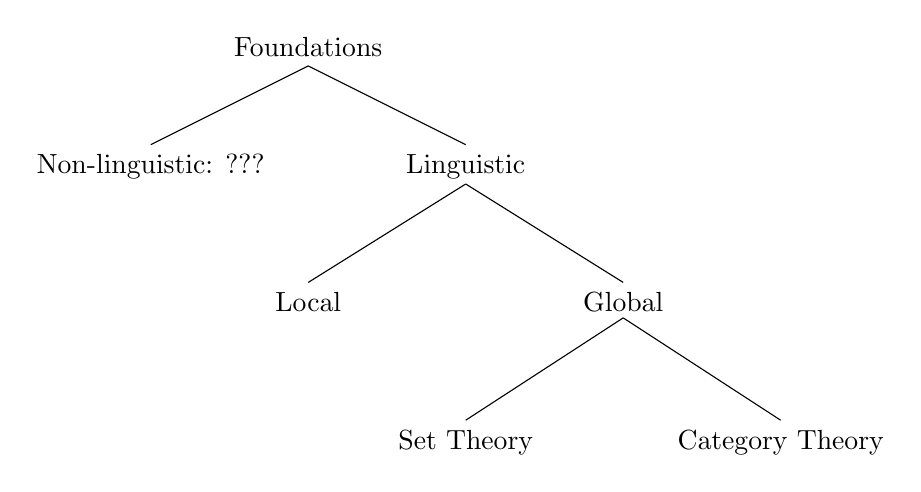
\begin{tikzpicture}
\draw (2,-1) -- (4,0);
\draw (6,-1) -- (4,0);
\draw (6,-1.5) -- (4,-2.75);
\draw (6,-1.5) -- (8,-2.75);
\draw (8,-3.2) -- (6,-4.5);
\draw (8,-3.2) -- (10,-4.5);
\node[align=center, above] at (4.0,0)%
{Foundations};
\node[align=center, below] at (2,-1)%
{Non-linguistic: ???};
\node[align=center, below] at (6,-1)%
{Linguistic};
\node[align=center, below] at (4,-2.75)%
{Local};
\node[align=center, below] at (8,-2.75)%
{Global};
\node[align=center, below] at (6,-4.5)%
{Set Theory};
\node[align=center, below] at (10,-4.5)%
{Category Theory};
\end{tikzpicture}


\end{frame}


\begin{frame}{General argument against linguistic foundations}

\begin{itemize}
\item Global: ZFC, ETCS, CCAF.  There is a fixed language and a fixed
  criterion of identity.
\item Local: SFAM, Bell's local mathematics, model theory, Bourbaki
  style structuralism.
\end{itemize}


\end{frame}
\begin{frame}{Foundations without language: MLTT, HoTT, UF}

Four types of judgments

\bigskip
\begin{tabular}{ll}
$\Gamma\vdash A\;\mathbf{Type}$ & $A$ is a type \\
$\Gamma\vdash A=B\;\mathbf{Type}$ & $A$ and $B$ are the same type \\
$\Gamma\vdash a:A$ & $a$ is a term of type $A$ \\
$\Gamma\vdash a=b:A$ & $a$ and $b$ are the same term of type $A$
\end{tabular}



\end{frame}

\begin{frame}

\begin{mathpar}
 \inferrule*[right=$\mathtt{Id}$-form]
  {\Gamma \vdash A \colon \mathcal{U} \\ \Gamma \vdash a \colon A \\ \Gamma \vdash b \colon A}
  {\Gamma \vdash a=_Ab \colon \mathcal{U}}
\and
  \inferrule*[right=$\mathtt{Id}$-intro]
  {\Gamma \vdash A \colon \mathcal{U} \\ \Gamma \vdash a \colon A}
  {\Gamma \vdash \mathtt{refl}_a \colon a=_Aa}
\and
  \inferrule*[right=$\mathtt{Id}$-elim]
  {\Gamma, x \colon A, y \colon A, p \colon x=_Ay \vdash C \colon \mathcal{U} \\
   \Gamma, z \colon A \vdash d(z) \colon C(z,z,\mathtt{refl}_z)}
  %\Gamma \vdash a \colon A \\ \Gamma \vdash b \colon A \\ \Gamma \vdash p' \colon a=_Ab}
  {\Gamma \vdash D \colon \underset{a,b,p'}{\Pi} C(a,b,p')}
\and
  \inferrule*[right=$\mathtt{Id}$-comp]
  { \Gamma, x \colon A, y \colon A, p \colon x=_Ay \vdash C \colon \mathcal{U} \\
   \Gamma, z \colon A \vdash d \colon C(z,z,\mathtt{refl}_z) \\
   \Gamma \vdash a \colon A}
  {\Gamma \vdash D(a,a,\mathtt{refl}_a)=d(a) \colon C(a,a,\mathtt{refl}_a)}
\end{mathpar}


\end{frame}
\begin{frame}

\begin{table}[htb]
  \centering
 \begin{tabular}{lllll}
   \hline
   \textbf{Type Theory} && \textbf{Logic} & \textbf{Set Theory} & \textbf{HoTT}\\ %\addlinespace[2pt]
   \hline
   $A$ && proposition & set & space\\ %\addlinespace[2pt]
   $a:A$ && proof & element & point \\ %\addlinespace[2pt]
   $B(x)$ && predicate & family of sets & fibration \\ %\addlinespace[2pt]
   $b(x) : B(x)$ && conditional proof & family of elements & section\\ %\addlinespace[2pt]
   $0, 1$ && $\bot, \top$ & $\emptyset, \{ \emptyset \}$ & $\emptyset, *$\\ %\addlinespace[2pt]
   $A + B$ && $A\vee B$ & disjoint union & coproduct\\ %\addlinespace[2pt]
   $A\times B$ && $A\wedge B$ & set of pairs & product space\\ %\addlinespace[2pt]
   $A\to B$ && $A\Rightarrow B$ & set of functions & function space\\ %\addlinespace[2pt]
   $\underset{x \colon A}{\Sigma} B(x)$ &&  $\exists x \in A B(x)$ & disjoint sum & total space\\ %\addlinespace[2pt]
   $\underset{x \colon A}{\Pi} B(x)$ &&  $\forall x \in A B(x)$ & product & space of sections\\ %\addlinespace[2pt]
   $\mathsf{Id}_{A}(x,y)$ && x = y & $\{ \langle x,x\rangle \mid x\in A\}$ & path space $A^I$ \\ %\addlinespace[2pt]
   \hline
  \end{tabular}
  \caption{Points of view of Type Theory}\label{tab:pov}
\end{table}


\end{frame}

\begin{frame}{Univalence for Dummies}

  Overheard: ``Isomorphism \emph{is} Identity''

\bigskip

\[
\mathtt{isEquiv} (f) = \underset{x \colon A}{\Pi} \mathtt{isContr}( \mathtt{hFib} (f,x))
\]

\[
\mathtt{univ} \colon \underset{A,B \colon \mathcal{U}}{\Pi} \mathtt{isEquiv} (\mathtt{idtoequiv})
\]
where \texttt{idtoequiv} is the canonical map guaranteed by
induction. Or in a more informal manner:
\[
(A = B) \simeq (A \simeq B) 
\]

\textcolor{green}{YES:} Isomorphism is Isomorphic to Identity

\end{frame}

\begin{frame}{Univalence as a transport principle}

  The Univalence Axiom should, at least from a logical/foundational
  point of view, be viewed as a ``transport'' principle: it allows
  transport of any proof about a ``structure'' (i.e.\ a type) to any
  ``structure'' that is equivalent to it, via the identity type.

  Type-theoretic properties are invariant under types for which a
  proof of identity can be produced, and therefore properties will be
  invariant under equivalent types too.


\end{frame}



\begin{frame}{Connecting FOLDS and UF} 

  Using (Ahrendt, Kapulkin, Shulman 2013), we can show:


\begin{theorem} Every expressible property of an object in a
  category is invariant under isomorphism. \end{theorem}


\begin{proof}
  Take a category $\mathcal{C}$ with object type $C$. A property of an
  object in $\2C$ is a type $C \rightarrow \textbf{Prop}$. Suppose
  $C(a)$ holds for some $a \colon C$, i.e. there exists a term (proof)
  $p \colon C(a)$ and suppose also that there is an isomorphism
  between $a$ and $b$, i.e. a term $\eta \colon a \cong b$. Now, by
  the condition, the canonical map $\mathtt{idtoiso}(a,b)$ has a
  quasi-inverse $\mathtt{isotoid}(a,b)$. Thus we get a term $$
  \epsilon =_{\text{df}} \mathtt{isotoid}(a,b)(\eta) \colon
  \mathtt{Id}_C (a,b)$$ Since we now have a proof of identity we may
  transfer any property that we can express of $a$ along it and
  construct a proof that that property holds also of the other
  identificand. More precisely we use the $\mathtt{transport}$
  function to transfer the proof $p$ along $\epsilon$, thus getting a
  term $\mathtt{transport}(\epsilon)(p) \colon C(b)$, as required.
\end{proof}

\end{frame}


\begin{frame}{Connecting FOLDS and UF}


  \textbf{Theorem} (Makkai-Tsementzis) Let $S,T$ be Kan
  complexes. Then $S$ and $T$ are homotopy equivalent if and only if
  $i^*S \simeq_{\Delta_+^{\text{op}}} i^*T$ (i.e. if and only if
  $i^*S$ and $i^*T$ are FOLDS-equivalent as FOLDS
  $\Delta_+^{\text{op}}$-structures.)

  \end{frame}




\end{document}



